% \input{\pSections "sec-writ-large"}

\section{Writ Large}

%     %     %     %     %     %     %     %     %
\subsection{Radar Images of Satellite}
\begin{frame}\frametitle{Sealing the Mesh}
Boo
\end{frame}
		%
%     %     %     %     %     %     %     %     %
\subsection{Domains}
\begin{frame}{Domain Visualizations}
    \centering
    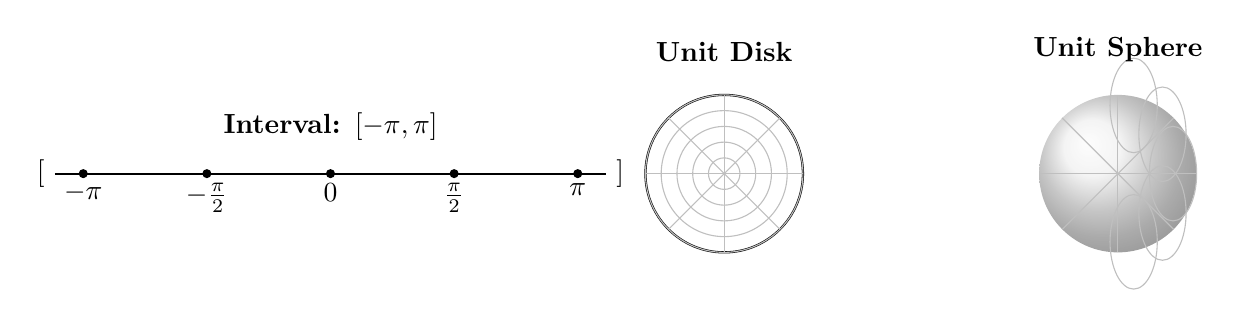
\begin{tikzpicture}
        % Left: Interval [-pi, pi]
        \begin{scope}[xshift=-5cm]
            \draw[thick] (-3.14,0) -- (3.14,0); % Solid line
            \draw[thick] (-3.5,0) node[left] {$[$} -- (-3.14,0);
            \draw[thick] (3.14,0) -- (3.5,0) node[right] {$]$};
            \foreach \x/\label in {-3.14/$-\pi$, -1.57/$-\frac{\pi}{2}$, 0/$0$, 1.57/$\frac{\pi}{2}$, 3.14/$\pi$}
                \draw[fill=black] (\x,0) circle (0.05) node[below] {\label};
            \node[above] at (0,0.3) {\textbf{Interval: \([- \pi, \pi]\)}};
        \end{scope}

        % Center: Unit Disk (Polar Grid)
        \begin{scope}
            \draw[thick] (0,0) circle (1cm); % Outer circle
            \foreach \r in {0.2,0.4,0.6,0.8,1}
                \draw[gray!50, thin] (0,0) circle (\r cm); % Concentric circles
            \foreach \a in {0,45,90,135,180,225,270,315}
                \draw[gray!50, thin] (0,0) -- (\a:1cm); % Radial lines
            \node[above] at (0,1.3) {\textbf{Unit Disk}};
        \end{scope}

        % Right: Unit Sphere (3D Mesh)
        \begin{scope}[xshift=5cm]
            \shade[ball color=gray!20, opacity=0.6] (0,0) circle (1cm); % Sphere shading
            \foreach \phi in {-60,-30,0,30,60}
                \draw[gray!50, thin] (\phi:1cm) arc (0:360:0.3 and 0.6); % Latitude lines
            \foreach \theta in {0,45,...,360}
                \draw[gray!50, thin] (\theta:1cm) -- (\theta:0cm); % Longitude lines
            \node[above] at (0,1.3) {\textbf{Unit Sphere}};
        \end{scope}
    \end{tikzpicture}
\end{frame}

\begin{frame}{Domain Visualizations}
    \centering
    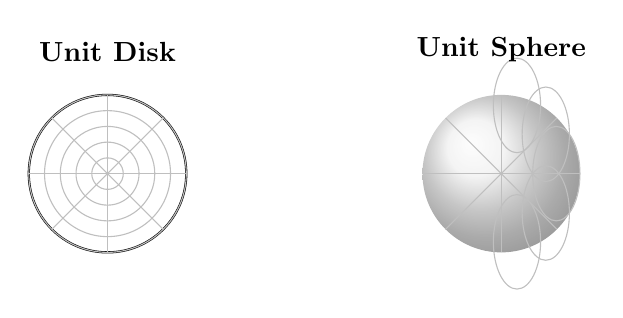
\begin{tikzpicture}

        % Center: Unit Disk (Polar Grid)
        \begin{scope}
            \draw[thick] (0,0) circle (1cm); % Outer circle
            \foreach \r in {0.2,0.4,0.6,0.8,1}
                \draw[gray!50, thin] (0,0) circle (\r cm); % Concentric circles
            \foreach \a in {0,45,90,135,180,225,270,315}
                \draw[gray!50, thin] (0,0) -- (\a:1cm); % Radial lines
            \node[above] at (0,1.3) {\textbf{Unit Disk}};
        \end{scope}

        % Right: Unit Sphere (3D Mesh)
        \begin{scope}[xshift=5cm]
            \shade[ball color=gray!20, opacity=0.6] (0,0) circle (1cm); % Sphere shading
            \foreach \phi in {-60,-30,0,30,60}
                \draw[gray!50, thin] (\phi:1cm) arc (0:360:0.3 and 0.6); % Latitude lines
            \foreach \theta in {0,45,...,360}
                \draw[gray!50, thin] (\theta:1cm) -- (\theta:0cm); % Longitude lines
            \node[above] at (0,1.3) {\textbf{Unit Sphere}};
        \end{scope}
    \end{tikzpicture}
\end{frame}

%     %     %     %     %     %     %     %     %
\subsection{Approximation}
\begin{frame}{Fourier and Extensions to 2- and 3-D}
    \centering
    $\fourier$
    \vspace{1em}
    \textit{From periodic functions in 1D to radial and angular decompositions in 2D and 3D.}
\end{frame}
	
\begin{frame}{Why We Love Fourier for Smooth Functions}
    \bl{Smooth Functions, Beautiful Representations}
    \begin{itemize}
        \item \bl{Weierstrass Approximation Theorem:} 
        Any continuous function on \([a, b]\) can be uniformly approximated by polynomials. Fourier provides a similar approximation, using trigonometric bases instead of polynomials.
        
        \item \bl{Riesz-Fischer Theorem:} 
        Fourier coefficients \((a_n, b_n)\) belong to \(l^2\) space, guaranteeing convergence in the \(L^2\) sense. This bridges the gap between smoothness and square-integrability.

        \item \bl{Uniform Convergence for Smooth Periodic Functions:} 
        For sufficiently smooth functions (\(C^\infty\) or \(C^k\)), Fourier series converge uniformly, ensuring no oscillatory artifacts (Gibbs phenomenon disappears).

        \item \bl{Orthogonality of Basis:} 
        Sines and cosines form an orthogonal basis in \(L^2\), enabling direct computation of coefficients via projection (Parseval's theorem quantifies energy distribution).

        \item \bl{Spectral Insights:} 
        Decomposes a function into frequency components, making smoothness and structure explicit. High smoothness = rapid Fourier coefficient decay.

        \item \bl{Compact Representation:} 
        Smooth functions require fewer terms for accurate approximation. High efficiency for practical computation and storage.

        \item \bl{Universality:} 
        Fourier's reach extends to PDEs, signal processing, and quantum mechanics. Smooth functions unlock the full power of these tools.
    \end{itemize}
    \vspace{1em}
    \bl{Takeaway:} Fourier connects smoothness, convergence, and representation, offering unmatched clarity and utility for periodic and localized phenomena.
\end{frame}

\begin{frame}{Fourier and Extensions to 2- and 3D}
    \centering
    \renewcommand{\arraystretch}{2.0}
    \setlength{\tabcolsep}{10pt} % Adjust column spacing
    
    \begin{tabular}{@{} l c @{}} % Align left and center without extra spacing
        \textcolor{blue}{\bl{1D:}} & 
        \( \displaystyle f(\theta) = \sum_{n=-\infty}^{\infty} a_{n} \fourier \) \\[1em]

        \textcolor{blue}{\bl{2D:}} & 
        \( \displaystyle f(r, \theta) = \sum_{n=0}^{\infty}\sum_{m=-n}^{n,2} a_{n}^{m} \mg{R_n^m(r)}  \fourier  \) \\[1em]

        \textcolor{blue}{\bl{3D:}} & 
        \( \displaystyle 
        f(r, \theta, \phi) = 
        \sum_{n=0}^{\infty}\sum_{m=-n}^{n} 
        a_{n}^{m} \mg{\sqrt{\frac{(2m+1)(m-n)!}{4\pi (m+n)!}} 
        P_l^m(\cos \theta)} \fourier 
        \)
    \end{tabular}
\end{frame}
	
\begin{frame}{Fourier and Extensions to 2- and 3D}
    \begin{itemize}
        \item \href{https://mathworld.wolfram.com/FourierSeries.html}{\bl{1D Fourier Series:}} Decomposes a periodic function \(f(\theta)\) into a sum of complex exponentials with coefficients \(a_n\) capturing the amplitudes of each frequency component.
        \item \href{https://mathworld.wolfram.com/ZernikePolynomial.html}{\bl{2D Fourier-Bessel:}} Extends Fourier analysis to two dimensions using radial functions \(R_n^m(r)\), often employed in circular domains or optical applications.
        \item \href{https://mathworld.wolfram.com/SphericalHarmonic.html}{\bl{3D Spherical Harmonics:}} Represents functions on a sphere using harmonics \(Y_l^m(\theta, \phi)\) and radial components \(R_l(r)\), crucial in fields like quantum mechanics and gravitational modeling.
    \end{itemize}
\end{frame}

%\begin{frame}{The first few Zernike disk polynomials}
%\begin{table}[htp]
%%\caption{The first few Zernike disk polynomials. The parameter $n$ specifies the order; the parameter $m$ the angular frequency.}
%		\begin{center}
%			\begin{tabular}{c|ccccccccc}
%				%
%				$n$ \\
%				%
%				$\raisebox{12pt}{0}$ 
%				&&&&&\includegraphics[ width = 1cm ]{ \pBitbucketStrangeEps/sf/zernike/0300-pyramid-00-00.eps} \\
%				%
%				$\raisebox{12pt}{1}$ 
%				  &&&&\includegraphics[ width = 1cm ]{ \pBitbucketStrangeEps/sf/zernike/0300-pyramid-01--01.eps} &&
%				      \includegraphics[ width = 1cm ]{ \pBitbucketStrangeEps/sf/zernike/"0300-pyramid-01-01.eps"} \\
%				%
%				$\raisebox{12pt}{2}$ 
%				  &&&\includegraphics[ width = 1cm ]{ \pBitbucketStrangeEps/sf/zernike/"0300-pyramid-02--02".eps} &&
%				     \includegraphics[ width = 1cm ]{ \pBitbucketStrangeEps/sf/zernike/"0300-pyramid-02-00".eps} &&
%				     \includegraphics[ width = 1cm ]{ \pBitbucketStrangeEps/sf/zernike/"0300-pyramid-02-02".eps} \\
%				%
%				$\raisebox{12pt}{3}$ 
%				  &&\includegraphics[ width = 1cm ]{ \pBitbucketStrangeEps/sf/zernike/"0300-pyramid-03--03".eps} &&
%				    \includegraphics[ width = 1cm ]{ \pBitbucketStrangeEps/sf/zernike/"0300-pyramid-03--01".eps} &&
%				    \includegraphics[ width = 1cm ]{ \pBitbucketStrangeEps/sf/zernike/"0300-pyramid-03-01".eps} &&
%				    \includegraphics[ width = 1cm ]{ \pBitbucketStrangeEps/sf/zernike/"0300-pyramid-03-03".eps} \\
%				%
%				$\raisebox{12pt}{4}$ 
%				  & \includegraphics[ width = 1cm ]{ \pBitbucketStrangeEps/sf/zernike/"0300-pyramid-04--04".eps} &&
%				    \includegraphics[ width = 1cm ]{ \pBitbucketStrangeEps/sf/zernike/"0300-pyramid-04--02".eps} &&
%				    \includegraphics[ width = 1cm ]{ \pBitbucketStrangeEps/sf/zernike/"0300-pyramid-04-00".eps} &&
%				    \includegraphics[ width = 1cm ]{ \pBitbucketStrangeEps/sf/zernike/"0300-pyramid-04-02".eps} &&
%				    \includegraphics[ width = 1cm ]{ \pBitbucketStrangeEps/sf/zernike/"0300-pyramid-04-04".eps} \\\hline
%				%
%				& 4 & 3 & 2 & 1 & 0 & 1 & 2 & 3 & 4 \\
%				&&&&& $m$
%				%
%			\end{tabular}
%		\end{center}
%	\label{tab:zernike pyramid 3d}
%\end{table}%
%\end{frame}

\begin{frame}{Lowest Order Fourier Basic Functions}
    \centering
    \begin{columns}[c] % Center-align the columns
        % Left column: Even Parity
        \begin{column}{0.5\textwidth}
            \centering
            $f(-\theta) = f(\theta)$  \\[0.5em]
            \textbf{Even Parity} \\[0.5em]
            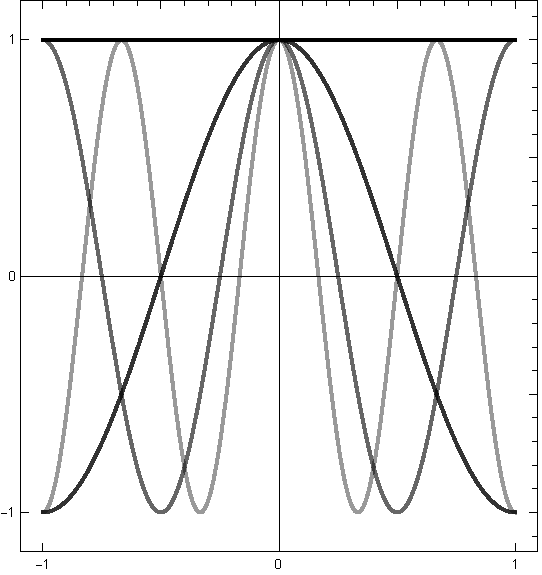
\includegraphics[width=0.8\linewidth]{\pLocalGraphics/fourier-cos.pdf}
        \end{column}

        % Right column: Odd Parity
        \begin{column}{0.5\textwidth}
            \centering
            $f(-\theta) = -f(\theta)$  \\[0.5em]
            \textbf{Odd Parity} \\[0.5em]
            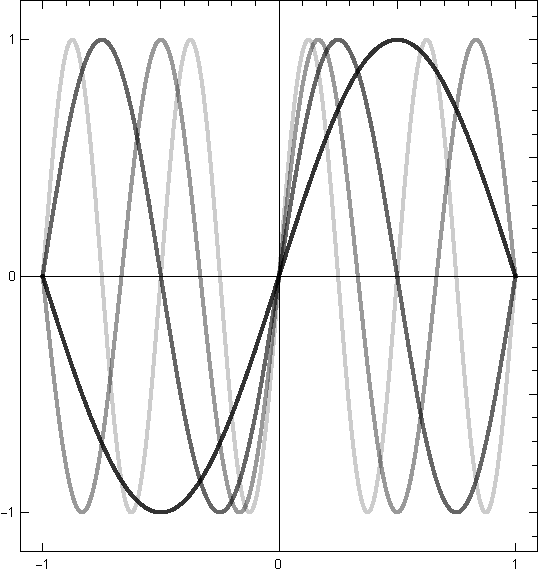
\includegraphics[width=0.8\linewidth]{\pLocalGraphics/fourier-sin.pdf}
        \end{column}
    \end{columns}
\end{frame}

\begin{frame}{Lowest Order Zernike Disk Polynomials}
    \centering
  	\setlength\extrarowheight{-6pt}
    %\renewcommand{\arraystretch}{-0.2} % Adjust row spacing
    \setlength{\tabcolsep}{3pt}       % Adjust column spacing
    \begin{tabular}{cccccccccc}
				$n$ \\
        %
 				$\raisebox{12pt}{0}$  &
        & & & & \includegraphics[width=1cm]{\pBitbucketStrangeEps/sf/zernike/0300-pyramid-00-00.eps} & & & & \\[-4pt]
        %
 				$\raisebox{12pt}{1}$  &
        & & & \includegraphics[width=1cm]{\pBitbucketStrangeEps/sf/zernike/0300-pyramid-01--01.eps} &
        & \includegraphics[width=1cm]{\pBitbucketStrangeEps/sf/zernike/0300-pyramid-01-01.eps} & & & \\[-4pt]
        %
 				$\raisebox{12pt}{2}$  &
        & & \includegraphics[width=1cm]{\pBitbucketStrangeEps/sf/zernike/0300-pyramid-02--02.eps} &
        & \includegraphics[width=1cm]{\pBitbucketStrangeEps/sf/zernike/0300-pyramid-02-00.eps} &
        & \includegraphics[width=1cm]{\pBitbucketStrangeEps/sf/zernike/0300-pyramid-02-02.eps} & & \\[-4pt]
        %
 				$\raisebox{12pt}{3}$  &
        & \includegraphics[width=1cm]{\pBitbucketStrangeEps/sf/zernike/0300-pyramid-03--03.eps} &
        & \includegraphics[width=1cm]{\pBitbucketStrangeEps/sf/zernike/0300-pyramid-03--01.eps} &
        & \includegraphics[width=1cm]{\pBitbucketStrangeEps/sf/zernike/0300-pyramid-03-01.eps} &
        & \includegraphics[width=1cm]{\pBitbucketStrangeEps/sf/zernike/0300-pyramid-03-03.eps} & \\[-4pt]
        %
				$\raisebox{12pt}{4}$  &
        \includegraphics[width=1cm]{\pBitbucketStrangeEps/sf/zernike/0300-pyramid-04--04.eps} &
        & \includegraphics[width=1cm]{\pBitbucketStrangeEps/sf/zernike/0300-pyramid-04--02.eps} &
        & \includegraphics[width=1cm]{\pBitbucketStrangeEps/sf/zernike/0300-pyramid-04-00.eps} &
        & \includegraphics[width=1cm]{\pBitbucketStrangeEps/sf/zernike/0300-pyramid-04-02.eps} &
        & \includegraphics[width=1cm]{\pBitbucketStrangeEps/sf/zernike/0300-pyramid-04-04.eps} \\[10pt]
        %
 				& -4 & -3 & -2 & -1 & 0 & 1 & 2 & 3 & 4 \\
				&&&&& $m$
    \end{tabular}
\end{frame}

%\begin{frame}{Fourier Basis Functions}
%    \centering
%    \begin{tikzpicture}
%        % Left Figure: Cosine Functions
%        \begin{axis}[
%            width=5.5cm, height=4cm, % Slightly reduce width to prevent overlap
%            title={\textbf{Cosine Basis Functions}},
%            xlabel={\(\theta\)}, ylabel={\(f(\theta)\)},
%            grid=both,
%            xtick={0,90,180,270,360},
%            xticklabels={\(0\), \(90^\circ\), \(180^\circ\), \(270^\circ\), \(360^\circ\)},
%            ymin=-1.2, ymax=1.2, % Tightened range for clarity
%            legend style={at={(0.5,1.05)}, anchor=south, legend columns=1, font=\tiny}
%        ]
%            \addplot[thick, blue] {cos(deg(0*x))};
%            \addlegendentry{\(\cos(0\theta)\)}
%            
%            \addplot[thick, red] {cos(deg(x))};
%            \addlegendentry{\(\cos(\theta)\)}
%            
%            \addplot[thick, green] {cos(deg(3*x))};
%            \addlegendentry{\(\cos(3\theta)\)}
%        \end{axis}
%
%        % Right Figure: Sine Functions
%        \begin{axis}[
%            at={(8cm,0)}, anchor=north west, % Manual positioning to avoid overlap
%            width=5.5cm, height=4cm, % Matching left plot size
%            title={\textbf{Sine Basis Functions}},
%            xlabel={\(\theta\)}, ylabel={\(f(\theta)\)},
%            grid=both,
%            xtick={0,90,180,270,360},
%            xticklabels={\(0\), \(90^\circ\), \(180^\circ\), \(270^\circ\), \(360^\circ\)},
%            ymin=-1.2, ymax=1.2,
%            legend style={at={(0.5,1.05)}, anchor=south, legend columns=1, font=\tiny}
%        ]
%            \addplot[thick, orange] {sin(deg(x))};
%            \addlegendentry{\(\sin(\theta)\)}
%            
%            \addplot[thick, purple] {sin(deg(2*x))};
%            \addlegendentry{\(\sin(2\theta)\)}
%            
%            \addplot[thick, cyan] {sin(deg(3*x))};
%            \addlegendentry{\(\sin(3\theta)\)}
%        \end{axis}
%    \end{tikzpicture}
%\end{frame}


%     %     %     %     %     %     %     %     %
\subsection{Quality of Fit}

\endinput  %  ==  ==  ==  ==  ==  ==  ==  ==  ==
